\section{Cross Sectional Estimation Frameworks}
\subsection{Ordinary Least Squares(OLS)}
\subsubsection{Simple OLS}

Model 0 is $Y_i = a+e_i$.

But given n pairs of observations on explanatory variable $X_i$ and dependent variable $Y_i$, we can have Model 1 by postulating that
\[
    Y_i = a + bX_i + e_i, \ i=1,2,\cdots,n,
\]
where $e_i$ is the noise.

Assumptions:
\begin{enumerate}
    \item $\mathbb{E}(e_i) = 0$ for every $i$
    \item $\mathbb{E}(e_i^2) = \sigma_e^2$
    \item $\mathbb{E}(e_i,e_j) = 0$ for every $i,j$
    \item $X_i,e_j$ are independednt for each $i,j$
    \item $e_i\sim \mathcal{N}(0,\sigma_e^2)$
\end{enumerate}

Least Sqaures: Minimizing the sum of squared errors:
\[
     \min_{\hat{a},\hat{b}}\sum_{i=1}^n e_i^2 = \sum_{i=1}^n(Y_i-\hat{a}-\hat{b}X_i)^2
\]

Set the first derivative of $a$ and $b$ as 0, we get:
\[
    \begin{aligned}
        \hat{a} &= \bar{Y} - \hat{b}\bar{X}\\
        \hat{b} &= \frac{\sum_{i=1}^nX_i(Y_i-\bar{Y})}{\sum_{i=1}^nX_i(X_i-\bar{X})}    \\
        &=\frac{\sum_{i=1}^n(X_i-\bar{X})(Y_i-\bar{Y})}{\sum_{i=1}^n(X_i-\bar{X})(X_i-\bar{X})}\\
        &=\frac{\mathbb{C}(Y,X)}{\mathbb{V}(X)}
    \end{aligned}
\] 

Properties of $\hat{a},\hat{b}$:

\[
    \begin{aligned}
        \hat{a} &\sim \mathcal{N}\left(a,\sigma_e^2\left(\frac{1}{n}+\frac{\bar{X}^2}{\sum_{i=1}^n\left(X_i-\bar{X}\right)^2}\right)\right)\\
        \hat{b} &\sim \mathcal{N}\left(b,\sigma_e^2\left(\frac{1}{\sum_{i=1}^n\left(X_i-\bar{X}\right)^2}\right)\right)
    \end{aligned}
\]
\begin{note}
    Because $\mathbb{E}(\hat{a}) = a$ ,$\mathbb{E}(\hat{b}) = b$, the $\hat{a}, \hat{b}$ are unbiased. Then Gauss-Markov Theorem states $\hat{a}$ and $\hat{b}$ has smallest variances, so $\hat{a}$ and $\hat{b}$ are efficient.
\end{note}

\subsubsection{Gauss-Markov Theorem}

\begin{theorem}{Gauss-Markov Theorem}
    states that among all linear and unbiased estimators, the OLS estimators $\hat{a}$ andb $\hat{b}$ have the minimum variances.
\end{theorem}

\subsubsection{OLS in Matrix}
Write model as $\mathbf{y} = \mathbf{X}\beta + \mathbf{e}$, by calculation, we get:
\[
    \hat{\beta} = (\mathbf{X}^{\prime}\mathbf{X})^{-1}\mathbf{X}^{\prime}\mathbf{y}
\]

\subsubsection{Hypothesis Testing}
Series of residuals:
\[
    \hat{e_i} = Y_i - \hat{a} - \hat{b}X_i, \ i=1,2,\cdots,n
\]

Testing null hypothesis $H_0: b =\beta (e.g.\ \beta = 0)$:
\[
    t_{n-2} = \frac{\hat{b}-\beta}{\hat{\sigma^e}\sqrt{\frac{1}{\sum_{i=1}^n(X_i-\bar{X})^2}}}
\]

Testing null hypothesis $H_0: a =\alpha (e.g.\ \alpha = 0)$:
\[
    t_{n-2} = \frac{\hat{a}-\alpha}{\hat{\sigma^e}\sqrt{\frac{1}{n}+\frac{\bar{X}^2}{\sum_{i=1}^n(X_i-\bar{X})^2}}}
\]

\begin{note}
    The denominators in testings are \textbf{standard errors} of $\hat{b}$ and $\hat{a}$.
\end{note}

\subsubsection{Consistent Properties of OLS}
\begin{enumerate}
    \item OLS $\hat{b}$ estimator is consistent: \[\lim_{n \to \infty} \hat{b} = b\]
    \item OLS $\hat{a}$ estimator is consistent: \[\lim_{n \to \infty} \hat{a} = a\]
\end{enumerate}

\subsubsection{Decomposition}
\begin{itemize}
    \item TSS: Total Sum of Squares
    \item ESS: Explained Sum of Squares
    \item RSS: Residual Sum of Squares
\end{itemize}

\[
    \begin{aligned}
        \mathrm{TSS} &= \sum_{i=1}^n(Y_i-\bar{Y})^2\\
        \mathrm{ESS} &= \sum_{i=1}^n(\hat{Y_i}-\bar{Y})^2\\
        \mathrm{RSS} &= \sum_{i=1}^n\hat{e_i}^2 = \sum_{i=1}^n(Y_i-\hat{Y})^2\\
        \mathrm{TSS} &= \mathrm{ESS} + \mathrm{RSS}\\
        R^2 &\coloneqq \frac{ESS}{TSS}
    \end{aligned}
\]

\subsubsection{Point Forecast and Confidence Interval}
The point forecast is 
\[
    \hat{Y_{n+1}} = \hat{a} + \hat{b}X_{n+1}
\]

With 95\% probability, the forecast value falls within the confidence interval bounded by
\[
    \hat{Y}_{n+1} \pm t_{n-2,97.5\%} \times \hat{\sigma_e}\sqrt{1+\frac{1}{n}+\frac{(X_{n+1}-\bar{X})^2}{\sum_{i=1}^n(X_i-\bar{X})^2}}
\]

\subsection{Discrete dependent variables}
\begin{itemize}
    \item Probit/logit model: used for binary dependent variables
    \item Multinomial probit/logit: Categorical dependent variables
    \item Ordered probit/logit: Discrete dependent variables
\end{itemize}

Probit:
\[
    \phi(X) = \mathbb{P}(Z\leq X) = \frac{1}{\sqrt{2\pi}}\int_{-\infty}^X \exp(-\frac{u^2}{2})du
\]

Logit:
\[
    \phi(X) = \mathbb{P}(Z\leq X) = \frac{1}{1+\exp(-k(X-X_0))}
\]

\begin{figure}[!ht]
	\centering
	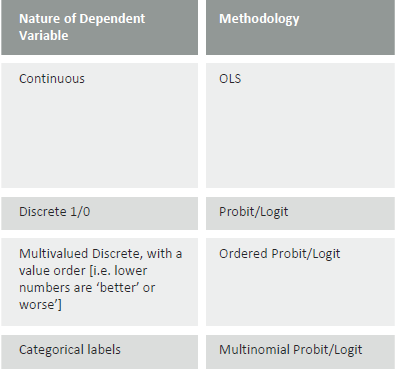
\includegraphics[width=\textwidth]{variables_method.png}
	\caption{Methodology roadmap}
\end{figure}
